\begin{ledgroupsized}[r]{120mm}%
\footnotesize%
\pstart%
\noindent\textbf{\"{U}berlieferung:}%
\pend%
\end{ledgroupsized}%
%
\begin{ledgroupsized}[r]{114mm}%
\footnotesize%
\pstart%
\parindent -6mm%
\makebox[6mm][l]{\textit{L}}%
Aufzeichnung: LH XXXVII 6 Bl. 3-4.
1 Bog. 2\textsuperscript{o}. Etwa \unitfrac{4}{5} S. auf Bl. 3~r\textsuperscript{o}.
Bl. 3~v\textsuperscript{o} und 4~r\textsuperscript{o} leer.
Die letzten 11 Z. auf Bl. 3~r\textsuperscript{o} sowie Bl. 4~v\textsuperscript{o} überliefern N.~63. % LH037,06_004v
\newline%
Cc 2, Nr. 1054 (tlw.)%
\pend%
\end{ledgroupsized}%
% \normalsize
% \vspace*{5mm}% PR: Abstand hier bitte kontrollieren !!!
%
\vspace{6mm}%
\count\Bfootins=1200
\count\Cfootins=1200
\count\Afootins=1200
\pstart%
\normalsize%
\noindent%
% [3~r\textsuperscript{o}]
[3~r\textsuperscript{o}] 
Sept. 1675%
\edtext{}{\lemma{}\Afootnote{\textit{Daneben, am Rand:} (1)}}\\
Modus coagulandi et tingendi Mercurium\protect\index{Sachverzeichnis}{mercurius} vulgi in aureum colorem.
Dissolve per 3. aut 6 horas in aqua pluviali\protect\index{Sachverzeichnis}{aqua pluvialis} $\oright$\textsuperscript{li} hungarici\protect\index{Sachverzeichnis}{vitriolum hungaricum} lib. II.
Filtretur dissolutio, et in vas ferreum infundatur, in qua coque igne carbonum \mercury \textsuperscript{rii}\protect\index{Sachverzeichnis}{mercurius} libram semis; donec maxima ex parte videatur congelatus, movendo semper et%
\edtext{}{\lemma{}\Afootnote{\textit{Am Rand:} verum\vspace{-4mm}}}
agitando strenue cum spatula\protect\index{Sachverzeichnis}{spatula} ferrea (ut scilicet \mercury \textsuperscript{ius}\protect\index{Sachverzeichnis}{mercurius} melius imbibat \raisebox{-4pt}{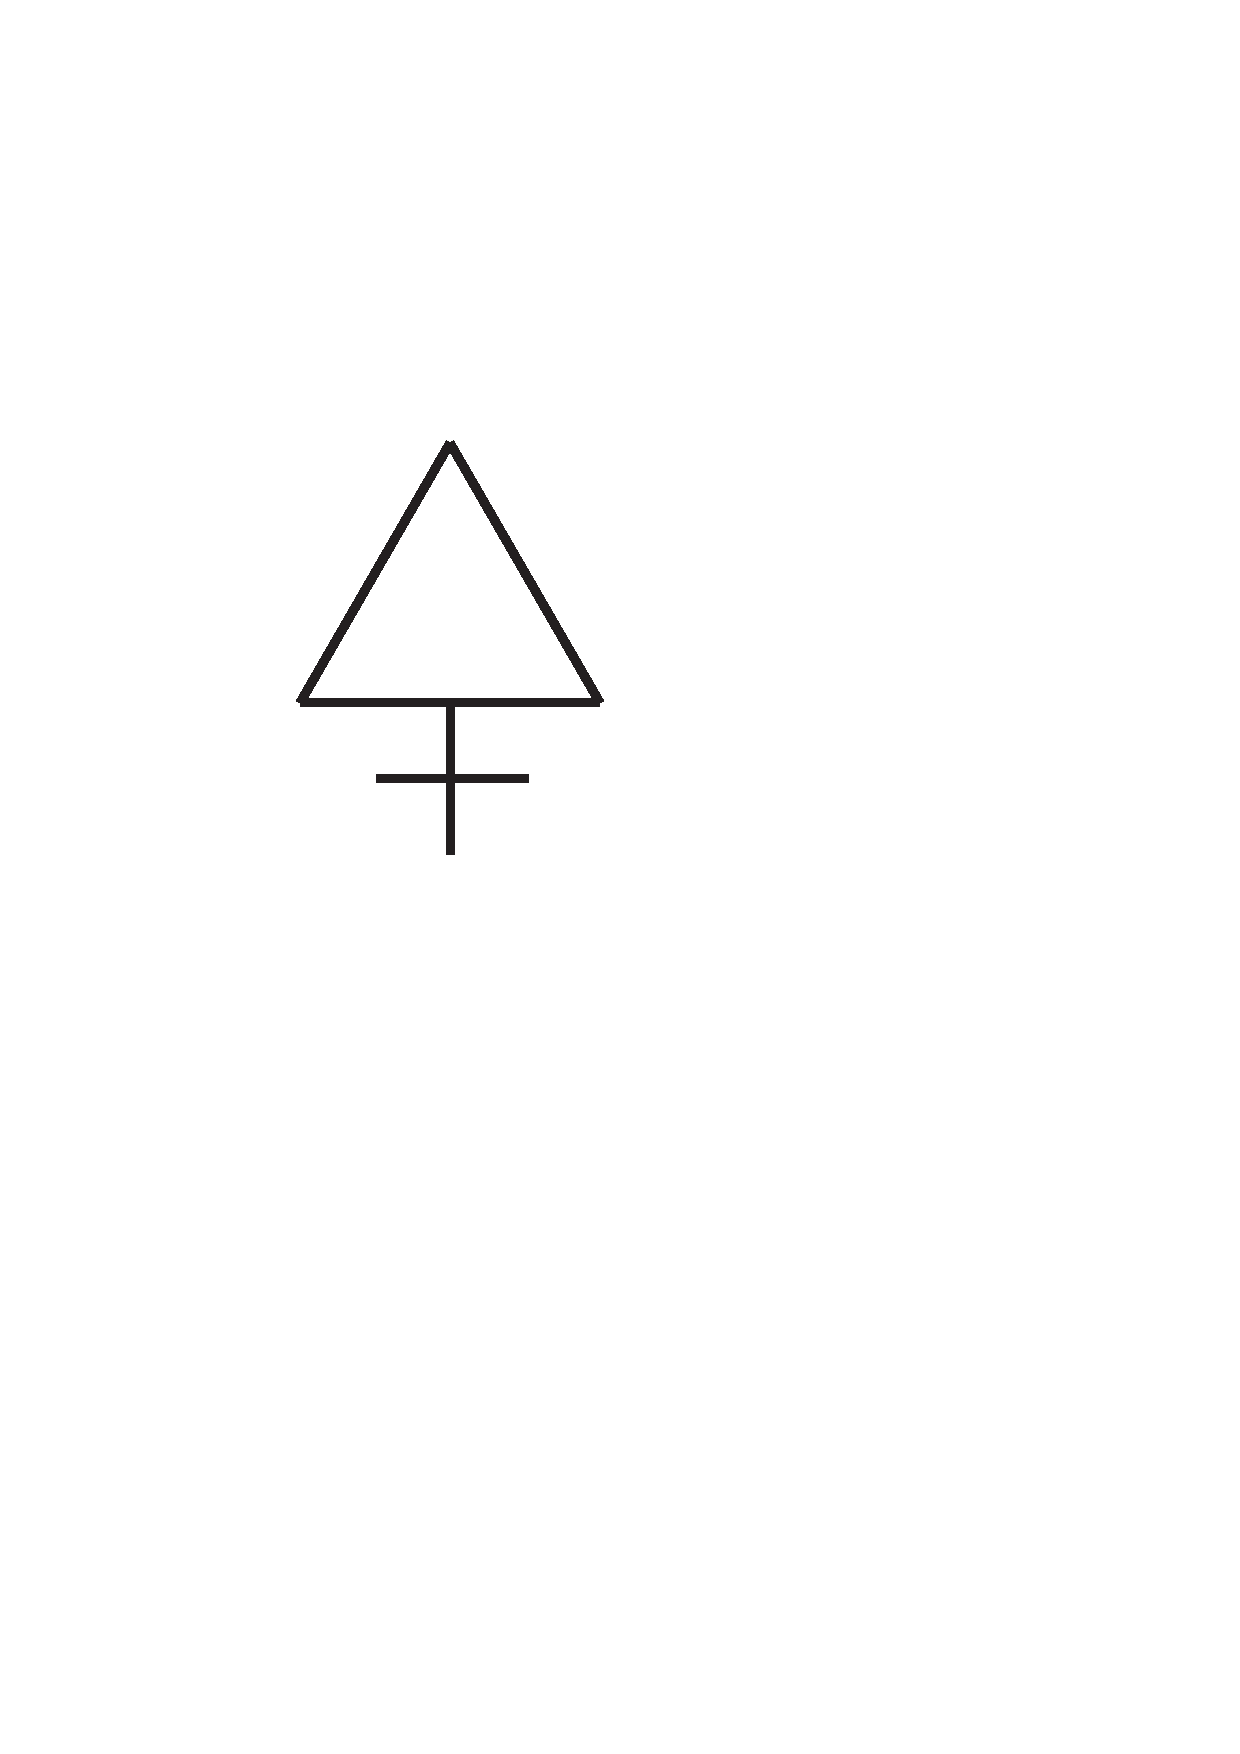
\includegraphics[width=0.02\textwidth]{images/sym-sulph.pdf}}\protect\index{Sachverzeichnis}{sulphur} acidum $\oright$\textsuperscript{li}\protect\index{Sachverzeichnis}{acidum vitrioli} quod est coagulativum \mercury \textsuperscript{ii}\protect\index{Sachverzeichnis}{mercurius} quemadmodum quoque omnes res acidae exempli gratia acetum\protect\index{Sachverzeichnis}{acetum} distillatum cum sale communi, aqua ferrea\protect\index{Sachverzeichnis}{aqua ferrea} etc.) tunc a Mercurio\protect\index{Sachverzeichnis}{mercurius} per inclinationem separa, et mercurium\protect\index{Sachverzeichnis}{mercurius} per corium Cervinum exprime ut incoagulatus transeat, et separetur a coagulato qui in corio remanebit, et incoagulatum \mercury \textsuperscript{ium}\protect\index{Sachverzeichnis}{mercurius} iterum coque in praedicta aqua et exprime et excoque donec totus coaguletur. Ex eo autem coagulato antequam indurescat forma parvos globulos, ac in crucibulum fortissimum immitte radicis\protect\index{Sachverzeichnis}{radix} Curcumae\protect\index{Sachverzeichnis}{curcuma} et Tutiae\protect\index{Sachverzeichnis}{tutia} simul pulverisatae et commissae ad crassitiem medii digiti stratum unum, cui impone globulorum stratum alium, rursusque de pulvere et de globulis stratum super stratum, donec repleatur crucibulum, cui operculum adde aut alterum crucibulum os contra os, luto probe munitum atque junctum quod in aere aperto ac solis radiis libere exicca, per
\edtext{tres aut}{\lemma{tres}\Bfootnote{\textit{(1)}\ ac \textit{(2)}\ aut \textit{L}}}
plures dies exiccato adde ignem rotae\protect\index{Sachverzeichnis}{ignis rotae} hoc est
\edtext{circumcirca, quem}{\lemma{circumcirca,}\Bfootnote{\textit{(1)}\ et \textit{(2)}\ quem \textit{L}}}
gradatim auge, et per duas aut tres horas sub finem sic intende, ut toto tempore crucibulum inferius candeat, postea sine ut sua sponte frigescant, et aperto crucibulo reperies tinctum Mercurium\protect\index{Sachverzeichnis}{mercurius}, cui si cum curcuma\protect\index{Sachverzeichnis}{curcuma} et Tutia\protect\index{Sachverzeichnis}{tutia} paulum saponis veneti\protect\index{Sachverzeichnis}{sapo venetus} adjicias, frater quidam roseae crucis dixit, quod fiet malleabilis ac liquefiet, ut inde vasa possint conflari. Amen. Nota quod de curcuma duplum Tutiae\protect\index{Sachverzeichnis}{tutia} aut triplum est adhibendum, et credo quod sextuplum non nocebit.
\pend%
\newpage
\pstart%
\textso{Papier}\protect\index{Sachverzeichnis}{Papier}\textso{ zu zurichten da{\ss} man} mit allerhand metall darauff schreiben und zeichnen kan.
\pend%
\pstart%
\textrecipe.\
Crura ovina erstlich gekocht, hernach gebrandt und zu pulver
\edtext{gestossen oder}{\lemma{gestossen}\Bfootnote{\textit{(1)}\ und \textit{(2)}\ oder \textit{L}}}
geschabet; mit diesem pulver das papier\protect\index{Sachverzeichnis}{Papier} trocken angerieben.
\pend%
\pstart%
Oder das papier\protect\index{Sachverzeichnis}{Papier} angefe\"{u}chtet, und das pulver mit milch oder hausen blassen\protect\index{Sachverzeichnis}{hausenblasen} auff einem reibestein zart gerieben, und also das papier\protect\index{Sachverzeichnis}{Papier} wenn es halb trocken damit uberstrichen
(+~daz metall soll seine farbe darauff lassen~+).
\pend%
\pstart%
\textso{Salis volatilis}\protect\index{Sachverzeichnis}{sal volatile} processus.
\textrecipe.\
Subsidentiam ab aqua vitae\protect\index{Sachverzeichnis}{aqua vitae}
\edtext{ex vino}{\lemma{ex vino}\Bfootnote{\textit{erg. L}}}
extractam exiccetur in umbra[,] post contundatur grosso modo et indatur retortae lutatae.%
\edtext{}{\lemma{}\Afootnote{\textit{Am Rand:} verum}}
Cui addatur rostrum quatuor pedibus longum, et rostro aptetur recipiens, tunc omnibus bene obturatis adhibeatur ignis per gradus, ita ut quatuor diebus perficiatur operatio: nota igne aperto et frigidissimo loco ac tempore fiat.
Rectificatur cum sale fixo\protect\index{Sachverzeichnis}{sal fixum} amalgama\protect\index{Sachverzeichnis}{amalgama}
miscendo\edtext{}{\lemma{}\Afootnote{\textit{Am Rand:} NB}}
et in arena sublimando, tunc demum
ex spiritu vini\protect\index{Sachverzeichnis}{spiritus vini} sublimando.
Medico cuidam egregio lucrosus hic processus.
\pend%
\count\Bfootins=1500
\count\Cfootins=1500
\count\Afootins=1500